%%%%%%%%%%%%%%%%%%%%%%%%%%%%%%%%%%%%%%%%%
% Lachaise Assignment
% LaTeX Template
% Version 1.0 (26/6/2018)
%
% This template originates from:
% http://www.LaTeXTemplates.com
%
% Authors:
% Marion Lachaise & François Févotte
% Vel (vel@LaTeXTemplates.com)
%
% License:
% CC BY-NC-SA 3.0 (http://creativecommons.org/licenses/by-nc-sa/3.0/)
% 
%%%%%%%%%%%%%%%%%%%%%%%%%%%%%%%%%%%%%%%%%

%----------------------------------------------------------------------------------------
%	PACKAGES AND OTHER DOCUMENT CONFIGURATIONS
%----------------------------------------------------------------------------------------

\documentclass{article}

%%%%%%%%%%%%%%%%%%%%%%%%%%%%%%%%%%%%%%%%%
% Lachaise Assignment
% Structure Specification File
% Version 1.0 (26/6/2018)
%
% This template originates from:
% http://www.LaTeXTemplates.com
%
% Authors:
% Marion Lachaise & François Févotte
% Vel (vel@LaTeXTemplates.com)
%
% License:
% CC BY-NC-SA 3.0 (http://creativecommons.org/licenses/by-nc-sa/3.0/)
% 
%%%%%%%%%%%%%%%%%%%%%%%%%%%%%%%%%%%%%%%%%

%----------------------------------------------------------------------------------------
%	PACKAGES AND OTHER DOCUMENT CONFIGURATIONS
%----------------------------------------------------------------------------------------

\usepackage{amsmath,amsfonts,stmaryrd,amssymb} % Math packages

\usepackage{enumerate} % Custom item numbers for enumerations

\usepackage[ruled]{algorithm2e} % Algorithms

\usepackage[framemethod=tikz]{mdframed} % Allows defining custom boxed/framed environments

\usepackage{listings} % File listings, with syntax highlighting
\lstset{
	basicstyle=\ttfamily, % Typeset listings in monospace font
}

%----------------------------------------------------------------------------------------
%	DOCUMENT MARGINS
%----------------------------------------------------------------------------------------

\usepackage{geometry} % Required for adjusting page dimensions and margins

\geometry{
	paper=a4paper, % Paper size, change to letterpaper for US letter size
	top=2.5cm, % Top margin
	bottom=3cm, % Bottom margin
	left=2.5cm, % Left margin
	right=2.5cm, % Right margin
	headheight=14pt, % Header height
	footskip=1.5cm, % Space from the bottom margin to the baseline of the footer
	headsep=1.2cm, % Space from the top margin to the baseline of the header
	%showframe, % Uncomment to show how the type block is set on the page
}

%----------------------------------------------------------------------------------------
%	FONTS
%----------------------------------------------------------------------------------------

\usepackage[utf8]{inputenc} % Required for inputting international characters
\usepackage[T1]{fontenc} % Output font encoding for international characters

\usepackage{XCharter} % Use the XCharter fonts

%----------------------------------------------------------------------------------------
%	COMMAND LINE ENVIRONMENT
%----------------------------------------------------------------------------------------

% Usage:
% \begin{commandline}
%	\begin{verbatim}
%		$ ls
%		
%		Applications	Desktop	...
%	\end{verbatim}
% \end{commandline}

\mdfdefinestyle{commandline}{
	leftmargin=10pt,
	rightmargin=10pt,
	innerleftmargin=15pt,
	middlelinecolor=black!50!white,
	middlelinewidth=2pt,
	frametitlerule=false,
	backgroundcolor=black!5!white,
	frametitle={Command Line},
	frametitlefont={\normalfont\sffamily\color{white}\hspace{-1em}},
	frametitlebackgroundcolor=black!50!white,
	nobreak,
}

% Define a custom environment for command-line snapshots
\newenvironment{commandline}{
	\medskip
	\begin{mdframed}[style=commandline]
}{
	\end{mdframed}
	\medskip
}

%----------------------------------------------------------------------------------------
%	FILE CONTENTS ENVIRONMENT
%----------------------------------------------------------------------------------------

% Usage:
% \begin{file}[optional filename, defaults to "File"]
%	File contents, for example, with a listings environment
% \end{file}

\mdfdefinestyle{file}{
	innertopmargin=1.6\baselineskip,
	innerbottommargin=0.8\baselineskip,
	topline=false, bottomline=false,
	leftline=false, rightline=false,
	leftmargin=2cm,
	rightmargin=2cm,
	singleextra={%
		\draw[fill=black!10!white](P)++(0,-1.2em)rectangle(P-|O);
		\node[anchor=north west]
		at(P-|O){\ttfamily\mdfilename};
		%
		\def\l{3em}
		\draw(O-|P)++(-\l,0)--++(\l,\l)--(P)--(P-|O)--(O)--cycle;
		\draw(O-|P)++(-\l,0)--++(0,\l)--++(\l,0);
	},
	nobreak,
}

% Define a custom environment for file contents
\newenvironment{file}[1][File]{ % Set the default filename to "File"
	\medskip
	\newcommand{\mdfilename}{#1}
	\begin{mdframed}[style=file]
}{
	\end{mdframed}
	\medskip
}

%----------------------------------------------------------------------------------------
%	NUMBERED QUESTIONS ENVIRONMENT
%----------------------------------------------------------------------------------------

% Usage:
% \begin{question}[optional title]
%	Question contents
% \end{question}

\mdfdefinestyle{question}{
	innertopmargin=1.2\baselineskip,
	innerbottommargin=0.8\baselineskip,
	roundcorner=5pt,
	nobreak,
	singleextra={%
		\draw(P-|O)node[xshift=1em,anchor=west,fill=white,draw,rounded corners=5pt]{%
		Question \theQuestion\questionTitle};
	},
}

\newcounter{Question} % Stores the current question number that gets iterated with each new question

% Define a custom environment for numbered questions
\newenvironment{question}[1][\unskip]{
	\bigskip
	\stepcounter{Question}
	\newcommand{\questionTitle}{~#1}
	\begin{mdframed}[style=question]
}{
	\end{mdframed}
	\medskip
}

%----------------------------------------------------------------------------------------
%	WARNING TEXT ENVIRONMENT
%----------------------------------------------------------------------------------------

% Usage:
% \begin{warn}[optional title, defaults to "Warning:"]
%	Contents
% \end{warn}

\mdfdefinestyle{warning}{
	topline=false, bottomline=false,
	leftline=false, rightline=false,
	nobreak,
	singleextra={%
		\draw(P-|O)++(-0.5em,0)node(tmp1){};
		\draw(P-|O)++(0.5em,0)node(tmp2){};
		\fill[black,rotate around={45:(P-|O)}](tmp1)rectangle(tmp2);
		\node at(P-|O){\color{white}\scriptsize\bf !};
		\draw[very thick](P-|O)++(0,-1em)--(O);%--(O-|P);
	}
}

% Define a custom environment for warning text
\newenvironment{warn}[1][Warning:]{ % Set the default warning to "Warning:"
	\medskip
	\begin{mdframed}[style=warning]
		\noindent{\textbf{#1}}
}{
	\end{mdframed}
}

%----------------------------------------------------------------------------------------
%	INFORMATION ENVIRONMENT
%----------------------------------------------------------------------------------------

% Usage:
% \begin{info}[optional title, defaults to "Info:"]
% 	contents
% 	\end{info}

\mdfdefinestyle{info}{%
	topline=false, bottomline=false,
	leftline=false, rightline=false,
	nobreak,
	singleextra={%
		\fill[black](P-|O)circle[radius=0.4em];
		\node at(P-|O){\color{white}\scriptsize\bf i};
		\draw[very thick](P-|O)++(0,-0.8em)--(O);%--(O-|P);
	}
}

% Define a custom environment for information
\newenvironment{info}[1][Info:]{ % Set the default title to "Info:"
	\medskip
	\begin{mdframed}[style=info]
		\noindent{\textbf{#1}}
}{
	\end{mdframed}
}
%----------------------------------------------------------------------------------------
%  References/Bibliography 
%----------------------------------------------------------------------------------------

\usepackage[round, sort&compress, authoryear]{natbib}

%----------------------------------------------------------------------------------------
%  Links
%----------------------------------------------------------------------------------------

\usepackage{hyperref}
\usepackage{url}
\usepackage{xcolor}
\hypersetup{
	colorlinks,
	linkcolor={blue!80!black},
	citecolor={blue!80!black},
	urlcolor={blue!80!black}
}
 % Include the file specifying the document structure and custom commands

%----------------------------------------------------------------------------------------
%	ASSIGNMENT INFORMATION
%----------------------------------------------------------------------------------------

\title{Problem Set \#1 } % Title of the assignment

\author{Mahyar Ebrahimitorki\\ \texttt{mahyar\_ebrahimi\_torki@yahoo.com}} % Author name and email address

\date{University of South Carolina --- \today} % University, school and/or department name(s) and a date

%----------------------------------------------------------------------------------------

\begin{document}

\maketitle % Print the title

%----------------------------------------------------------------------------------------
%	INTRODUCTION
%----------------------------------------------------------------------------------------

\section*{ A brief summary of research interest } % Unnumbered section

I am interested in behavioral economics in crisis period and analyzing decision makers' behaviors in any section of economy to reveal their accumulate effects.In this regard I like to dig into game theory, now-casting methods and working with big data. I think by using big data and employing method of game theory I can categorize people's decision, specially in crisis. In the following paragraph, I will elaborate on the path which guides me to develop aforementioned interest.\\
Working in market, among people without academic background, taught me great lessons. While working in accounting company as an accountant and financial advisor, majority of people asked me to increase their wealth and they all had suggestions more accurate and tenable than mine. So it made me to think in a different way than I used to. I always try to analyze economy and financial markets based on historical data and the most up-to-date one without paying attention to the market decision makers and main costumers, in general, to the people who play the main role in the market. But as I mentioned, nonacademic people who gave me great recommendations analyze market based on behavior rather than statistics. Therefore, I decided to find the more reliable way to analyze this important factor which lead me to game theory and big data.\\
For now-casting and monitoring economic conditions we need to use real-time data flow  in high volume \cite{bok2018macroeconomic} which is called big data and for analyzing this type of data programming and web-scraping skills are crucially important because data should be not only comprehensive  but also relevant. \\
In this regard, following initial formula summarize the raw idea which I mentioned in previous paragraph:
\\\textbf{phase one} is modeling decision makers' decisions in crisis by using game theory 
\begin{equation}
  D_{t} = d_{f} + d_{h} + d_{g} + d_{o} + d_{fi}
\end{equation}
% Math equation/formula
  In the first formula $D_{t}$ is total affections of decision makers in all sectors,$d_{f}$ is  firms decision makers affections on all sectors, $d_{h}$ is households decision makers affections on all sectors, $d_{g}$ is firms decision makers affections on all sectors, $d_{o}$ is overseas  decision makers affections on all sectors $d_{fi}$ is financial  decision makers affections on all sectors.For formula 1 we use "Five-sector model" \cite{buultjens2000excel} as shown in figure 1 and 2 
 \begin{figure}
  	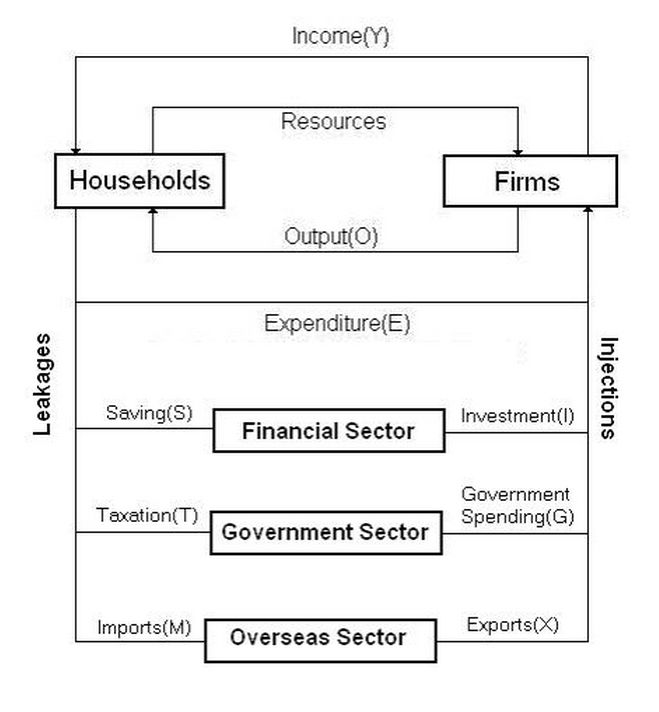
\includegraphics[width=\linewidth]{FiveSectorCircularFlowofIncomeModel.jpg}
  	\caption{five sector circular of income.}
  	\label{fig:1}
 \end{figure} 
  \begin{figure}
  	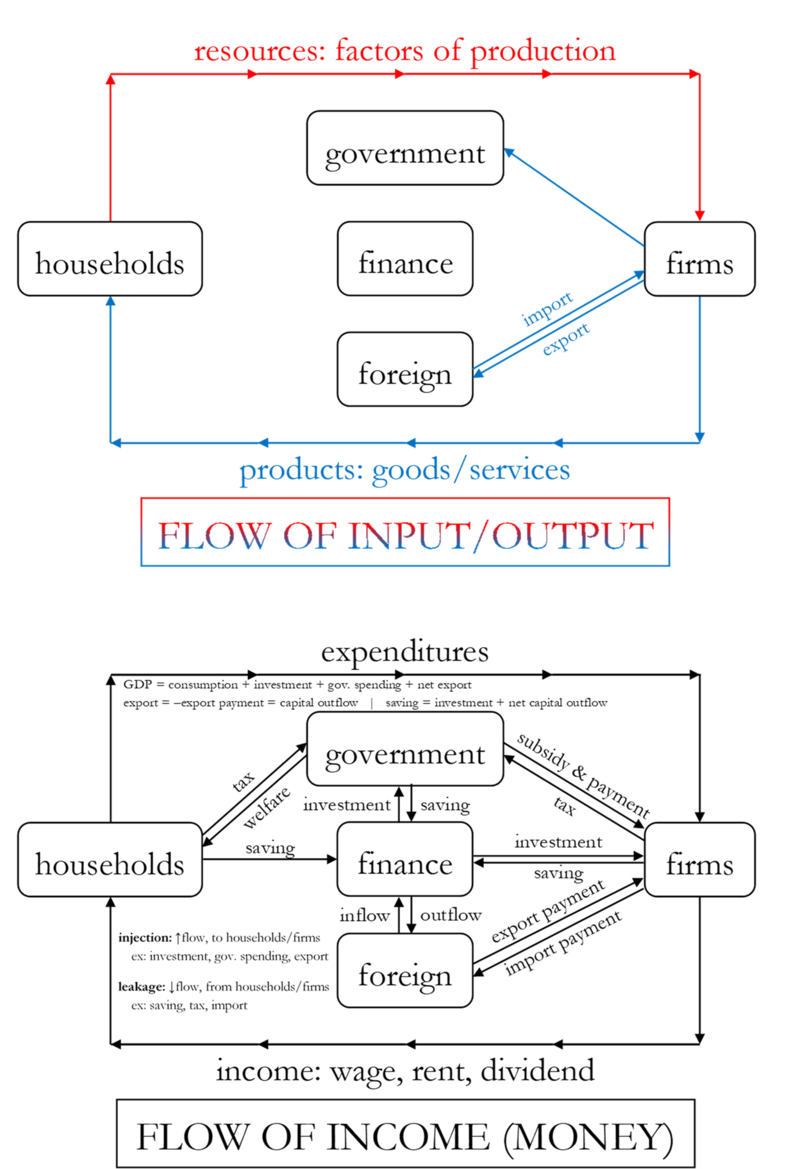
\includegraphics[width=\linewidth]{800px04circularflowdiagram.png}
  	\caption{Five sector circular flow}
  	\label{fig:1}
  \end{figure}
  	
  In the second phase, we nowcast the near future by using the outcome of first phase as follow: 
  \begin{equation}
  y_{t} = \beta_{1} D_{Tt} + \beta_{2} x_{t} + \varepsilon_{t}
  \end{equation}
  where $y_{t}$ is the economic variable of interest in the economy, $D_{Tt}$ is the outcome first step, and $x_{t}$ is the vector of other variables affecting the outcome variable. $\beta_{1}$ and $\beta_{2}$ are the coefficients and $\varepsilon_{t}$ is the vector of residuals. 
  	
\bibliographystyle{authordate1}
\bibliography{bibliography}


\end{document}
